\documentclass[12pt, a4paper]{book}

\usepackage[margin=2cm]{geometry}
\usepackage{tikz-cd}
\usepackage{mathtools}
\usepackage{graphicx}
\usepackage{xepersian}
\settextfont{Yas}
\begin{document}
\chapter{ترسیم‌های هندسی و استدلال}


\chapter{قضیه‌ی تالس، تشابه و کاربردهای آن}


\chapter{چند ضلعی‌ها}

\section[درس اول]{چند ضلعی‌ها و ویژگی‌هایی از آنها}

\textbf{تعریف:}
n
ضلعی شکلی است شامل 
(n $\geq$ 3) n
پاره‌خط متوالی که:\\
۱) هرپاره‌خطی، دقیقاً دو پاره‌خط دیگر را در نقاط انتهایی خودش قطع کند.\\
۲) هر دو پاره‌خط که در یک انتها مشترک‌اند، روی یک خط نباشند.

\subsection{قطر در چندضلعی‌ها}

در هر
n
ضلعی، هر پاره‌خط را که دو انتهای آن، دو رأس غیرمجاور باشند، قطر می‌نامند.

n
ضلعی 
$\mbox{A}_{1}\mbox{A}_{2} \dots \mbox{A}_{\mbox{n}}$
را در نظر می‌کیریم. از رأس 
$\mbox{A}_{1}$،
n-۱
قطر می‌توان رسم کرد.\\
با توجه به اینکه n رأس داریم، می‌توان گفت تعداد قطرها در n ضلعی با این فرمول به‌دست می‌آید:
\begin{minipage}{2 cm}
	\centering
	$\dfrac{n(n-3)}{2}$
\end{minipage}
\newline

\textbf{مثال:}

تعداد اقطار یک چند ضلعی ۳۵ است. از هر رأس این چندضلعی چند قطر می‌گذرد؟
\begin{flushleft}
$\dfrac{n(n-3)}{2} = 35 \Rightarrow x^2 -3x = 70 \Rightarrow (x-10)(x+7) = 0 \Rightarrow \left\{ \begin{array}{lll}
\fbox{$x =10$} & \mbox{ق‌ق} \\ x = -7 & \mbox{غ‌ق‌ق}
\end{array} \right.$
\end{flushleft}

تعداد اقطار یک چند ضلعی محدب از تعداد اضلاع آن ۴۲تا بیشتر است. این چند ضلعی چند قطر دارد؟
\begin{flushleft}
$\dfrac{n(n-3)}{2} = x+42 \Rightarrow x^2 -3x = 2x +84 \Rightarrow x^2 -5x -84 =0 \Rightarrow (x+7)(x-12) = 0  \Rightarrow \left\{ \begin{array}{lll}
\fbox{$x = 12$} & \mbox{ق‌ق} \\ x = -7 & \mbox{غ‌ق‌ق}
\end{array} \right.$
\end{flushleft}

مجموع تعداد اضلاع و اقطار یک 1 $\!+\!$ n ضلعی نصف اقطار یک 2n ضلعی است.  n چند است؟
\begin{flushleft}
$\dfrac{n+1(n+1-3)}{2} + n+1 = \dfrac{2n(2n-3)}{4} \Rightarrow \dfrac{n^2-n-2}{2}+ n+1 = \dfrac{4n^2-6n}{4} \Rightarrow \dfrac{n^2-n-2+2n+2}{2} = \dfrac{2n^2-3n}{2} \Rightarrow n^2+n = 2n^2 -3n \Rightarrow n^2 -4n = 0 \Rightarrow n(n-4) = 0  \Rightarrow \left\{ \begin{array}{lll}
n =0 & \mbox{غ‌ق‌ق} \\ \fbox{$n = 4$} & \mbox{ق‌ق}
\end{array} \right.$
\end{flushleft}

در یک ۱۰۰ ضلعی محدب تعداد اقطاری که از ۲ رأس غیرمجاور می‌گذرد چند تا است؟
\begin{flushleft}
$100 - 3 = 97 \qquad (2 \times 97) - 1 = 193$
\end{flushleft}

مجموع تعداد اقطار و اضلاع یک چند ضلعی محدب برابر ۱۲۰ است. تعداد اضلاع چند است؟
\begin{flushleft}
$\dfrac{n+1(n+1-3)}{2} + n = 120 \Rightarrow \dfrac{2n^2-3}{2} = 120 \Rightarrow n^2-n=240 \Rightarrow (n-16)(n+15) = 0 \Rightarrow \left\{ \begin{array}{lll}
 \fbox{$n = 16$} & \mbox{ق‌ق} \\ n =-17 & \mbox{غ‌ق‌ق}
\end{array} \right.$
\end{flushleft}

\subsection{چهارضلعی‌های مهم و ویژگی‌هایی  آنها}
\textbf{تعریف:}\\
۱- متوازی‌الاضلاع چهارضلعی‌ای است که، هر دو ضلع مقابل آن موازی باشند.\\
۲- مستطیل چهارضلعی‌ای است که ، همه‌ی زوایای آن قائمه باشند.\\
۳- لوزی چهارضلعی‌ای است که، هر چهارضلع آن هم‌اندازه باشند.\\
۴- مربع چهارضلعی‌ای است که، هر چهار ضلع آن هم‌اندازه و حداقل یک زاویه‌ی آن قائمه باشد.
\newline

با توجه به تعاریف بالا هر یک از عبارات زیر را نیز می‌توانیم توجیه کنیم: \smallskip\\
\textbf{الف)} مستطیل یک متوازی‌الاضلاع است.\\
\textbf{ب)} اگر در متوازی‌الاضلاع یکی از زوایا قائمه باشد، مستطیل است.\\
\textbf{پ)} لوزی یک متوازی‌الضلاع است\\
\textbf{ت)} مربع یک لوزی، مستطیل و متوازی‌الاضلاع است\\

\subsection{ویژگی‌هایی از متوازی‌الاضلاع}
متوازی‌الاضلاع چهارضلعی‌ای است که، هر دو ضلع مقابل آن موازی باشند.
\newline

\textbf{قضیه ۱:} هر در متوازی‌الاضلاع هر دو ضلع مقابل هم‌اندازه‌اند.

	\begin{minipage}{.7\textwidth}
		\centering فرض: 
		$AB \parallel CD, \; AD \parallel BC$
		\qquad حکم:
		$AB = CD, \; AD = BC$
	\begin{flushleft}
			$ \left. \begin{array}{rll}
		(AB \parallel CD, \, \text{مورب} \, BD ) \rightarrow \widehat{D}_1 = \widehat{B}_1 \\ (AD \parallel BC, \, \text{مورب} \, BD ) \rightarrow \widehat{D}_2 = \widehat{B}_2 \\ AC =AC
		\end{array} \right\} \xrightarrow{\text{زض‌ز}} \triangle ABC \cong  \triangle ADC 
		\Rightarrow AB = CD \, , \, AD = BC$
	\end{flushleft}
\end{minipage}
\begin{minipage}{.28\textwidth}
	\begin{flushleft}
		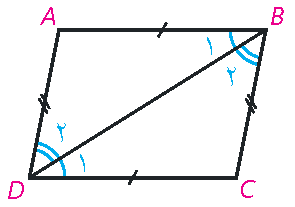
\includegraphics{"Shapes/Fasl - 3/Dars 1/qazie 1.pdf"}
	\end{flushleft}
\end{minipage}
\newline \bigskip \bigskip

\textbf{عکس قضیه ۱:} اگر در یک چهارضلعی، اضلاع مقابل دوبه‌دو هم‌اندازه باشند، چهارضلعی متوازی‌الاضلاع است.

	\begin{minipage}{.73\textwidth}
		\centering
	فرض: 
	$AB = CD, \; AD = BC$
	\qquad حکم:
	$AB \parallel CD, \; AD \parallel BC$
	\begin{flushleft}
		$ \left. \begin{array}{lll}
			AB = CD \\ AD = BC \\ AC = AC
		\end{array} \right\} \xRightarrow{\mbox{زض‌ز}} \triangle ABC \cong  \triangle ADC 
		\Rightarrow \left. \begin{array}{lll}
			 \widehat{A}_1 = \widehat{C}_1 \Rightarrow AB \parallel CD\\ \widehat{A}_2 = \widehat{C}_2 \Rightarrow AD \parallel BC
		\end{array} \right.$
	\end{flushleft}
\end{minipage}
\begin{minipage}{.28\textwidth}
	\begin{flushleft}
		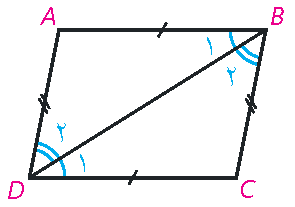
\includegraphics{"Shapes/Fasl - 3/Dars 1/qazie 1.pdf"}
	\end{flushleft}
\end{minipage} 
\newpage \bigskip

\textbf{قضیه ۲:} در متوازی‌الاضلاع هر دو زاویه‌ی مجاور مکمل‌اند.

\begin{minipage}{.7\textwidth}
	\centering فرض: 
	$AB \parallel CD, \; AD \parallel BC$
	\qquad حکم:
	$ \left. \begin{array}{rrr}
		\widehat{B}_2 + \widehat{C}_1 = 180^{\circ} \\ \widehat{C}_1 + \widehat{D} = 180^{\circ}
	\end{array} \right\}$
	\begin{flushleft}
		$(AB \parallel CD, \, \text{مورب} \, BC ) \rightarrow \left. \begin{array}{rll}
			  \widehat{C}_1 = \widehat{B}_1 \\ \widehat{B}_1 + \widehat{B}_2 = 180^{\circ} 
		\end{array} \right\} \rightarrow \widehat{C}_1 + \widehat{B}_2 = 180^{\circ} $
	
		$(AD \parallel BC, \, \text{مورب} \, CD ) \rightarrow \left. \begin{array}{rll}
			\widehat{D} = \widehat{C}_2 \\ \widehat{C}_1 + \widehat{C}_2 = 180^{\circ}
		\end{array} \right\} \rightarrow \widehat{D} + \widehat{C}_1 = 180^{\circ}$
	\end{flushleft}
\end{minipage}
\begin{minipage}{.28\textwidth}
	\begin{flushleft}
		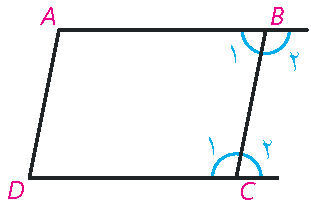
\includegraphics{"Shapes/Fasl - 3/Dars 1/qazie 2.pdf"}
	\end{flushleft}
\end{minipage}
\newline \bigskip \bigskip

\textbf{عکس قضیه ۲:} هر چهارضلعی که ر دو زاویه‌ی مجاور آن مکمل‌ باشند، متوازی‌الاضلاع است.

\begin{minipage}{.7\textwidth}
	\centering فرض: 
	$\left.
	\begin{array}{rrr}
		B_2 + D =180^{\circ} \\
		C_1 + D =180^{\circ} \\
		A + D = 180^{\circ} \\
		A + B_2 = 180^{\circ}
	\end{array}
	\right\}$
	\qquad حکم:
	$ \left. 
	\begin{array}{rrr}
		AB \parallel CD \\
		AD \parallel BC
	\end{array}
 \right\}$
	\begin{flushleft}
		$ \left.
		\begin{array}{rrr} 
			\widehat{C}_1 + \widehat{C}_2 = 180^{\circ} \\
			\widehat{C}_1 + \widehat{D} = 180^{\circ}
		\end{array}
	 \right\}
	  \rightarrow \widehat{D} = \widehat{C}_2 \Rightarrow AD \parallel BC$
	  
	  $\left.
	  \begin{array}{rrr} 
	  	\widehat{C}_1 + \widehat{B}_2 = 180^{\circ} \\
	  	\widehat{B}_1 + \widehat{B}_2 = 180^{\circ}
	  \end{array}
	  \right\}
	  \rightarrow \widehat{B}_1 = \widehat{C}_1 \Rightarrow AB \parallel CD$
	\end{flushleft}
\end{minipage}
\begin{minipage}{.28\textwidth}
	\begin{flushleft}
		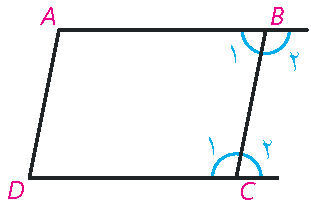
\includegraphics{"Shapes/Fasl - 3/Dars 1/qazie 2.pdf"}
	\end{flushleft}
\end{minipage}
\newline \bigskip \bigskip

\textbf{قضیه ۳:} در هر متوازی‌الضلاع، هر دو زاویه‌ی مقابل هم اندازه‌اند.

\begin{minipage}{.68\textwidth}
	\centering فرض: 
	$\left.
	\begin{array}{rrr}
		AB \parallel CD \\
		BC \parallel AD
	\end{array}
	\right\}$
	\qquad حکم:
	$ \left. 
	\begin{array}{rrr}
		\widehat{A} = \widehat{C} \\
		\widehat{B} = \widehat{D}
	\end{array}
 \right\}$
 \begin{flushright}
 	 بنا بر قضیه ۲ می‌توان نوشت:
 \end{flushright}
	\begin{flushleft}
		$ \left.
		\begin{array}{rrr} 
			\widehat{A} + \widehat{B} = 180^{\circ} \\
			\widehat{B} + \widehat{C} = 180^{\circ}
		\end{array}
	 \right\}
	 \rightarrow \widehat{A} = \widehat{C}
	 \qquad
	  \left.
	  \begin{array}{rrr} 
	  	\widehat{B} + \widehat{C} = 180^{\circ} \\
	  	\widehat{C} + \widehat{D} = 180^{\circ}
	  \end{array}
	  \right\}
	  \rightarrow \widehat{B} = \widehat{D}$
	\end{flushleft}
\end{minipage}
\begin{minipage}{.28\textwidth}
	\begin{flushleft}
		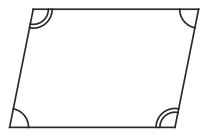
\includegraphics{"Shapes/Fasl - 3/Dars 1/qazie 3.pdf"}
	\end{flushleft}
\end{minipage}
\newline \bigskip \bigskip

\textbf{عکس قضیه ۳:} در هر یک چهارضلعی هر دو زاویه‌ی مقابل هم‌اندازه باشند، چهارضلعی متوازی‌الاضلاع است.

\begin{minipage}{.68\textwidth}
	\centering فرض: 
	$
		\widehat{A} = \widehat{C} = x \; , \; \widehat{B} = \widehat{C} = y
	$
	\qquad حکم:
	$ 
		ABCD 
	$ موازی‌الاضلاع است.
	\begin{flushleft}
		$ 
			x+y +x +y = 360^{\circ} \Rightarrow 2x + 2y = 360^{\circ} \Rightarrow x+y =180^{\circ}
		$
	\end{flushleft}
		هر دو زاویه‌ی مجاور مکمل‌اند،  بنابر عکس قضیه‌ ۲، ABCD متوازی‌الاضلاع است.
\end{minipage}
\begin{minipage}{.28\textwidth}
	\begin{flushleft}
		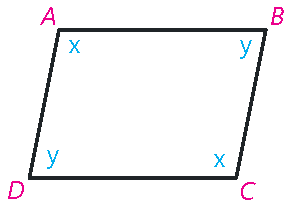
\includegraphics{"Shapes/Fasl - 3/Dars 1/qazie 3 ax.pdf"}
	\end{flushleft}
\end{minipage}
\newpage

\textbf{قضیه ۴:} در هر متوازی‌الاضلاع اقطار منصف یکدیگیرند.

\begin{minipage}{.68\textwidth}
	\centering فرض: 
	$
		AB \parallel CD \; , \; AD = BC
	$
	\qquad حکم:
	$ 
		OA = OC \; , \; OD = OB
	$
	\begin{flushleft}
		$ 
			\left. 
				\begin{array}{crr}
					\widehat{A}_1 = \widehat{C}_1 \\
					\widehat{B}_1 = \widehat{D}_1 \\
					AB = CD
				\end{array}
			\right\}
			\xRightarrow{\mbox{زض‌ز}} \triangle OAB \cong \triangle OCD \Rightarrow \left.
				\begin{array}{lll}
					OA = OC \\
					OB = OD
				\end{array}
			\right.
		$
	\end{flushleft}
\end{minipage}
\begin{minipage}{.28\textwidth}
	\begin{flushleft}
		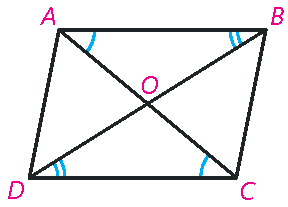
\includegraphics{"Shapes/Fasl - 3/Dars 1/qazie 4.pdf"}
	\end{flushleft}
\end{minipage}
\newline \bigskip \bigskip

\textbf{عکس قضیه ۴:} هر چهارضلعی‌ای که اقطارش منصف یکدیگر باشند، متوازی‌الاضلاع است.\\

\begin{minipage}{.68\textwidth}
	\centering فرض: 
	$
	 OA = OC \; , \; OD = OB
	$
	\qquad حکم:
	$ 
	AB \parallel CD \; , \; AD = BC
	$
	\begin{flushleft}
		$ 
		\left. 
		\begin{array}{crr}
			\widehat{O}_1 = \widehat{O}_2 \\
			OB = OD \\
			OA = OC
		\end{array}
		\right\}
		\xRightarrow{\mbox{ض‌زض}} \triangle OAB \cong \triangle OCD \Rightarrow \left.
		\begin{array}{cll}
			AB = CD \\
			\widehat{A}_1 = \widehat{C}_1 
		\end{array}
		\right.
		$
		$
		\widehat{A}_1 = \widehat{C}_1 \Rightarrow AB \parallel CD,\, \mbox{مورب} AC
		$
		
	\end{flushleft}
\end{minipage}
\begin{minipage}{.28\textwidth}
	\begin{flushleft}
		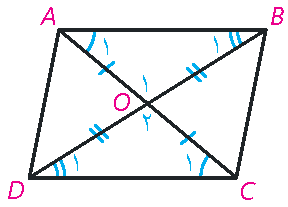
\includegraphics{"Shapes/Fasl - 3/Dars 1/qazie 4 ax.pdf"}
	\end{flushleft}
\end{minipage}
\newline \bigskip \bigskip

هر در چهاضلعی مه دو ضلع آن هم‌اندازه و موازی باشند.، متوازی‌الاضلاع است.

\begin{minipage}{.68\textwidth}
	\centering فرض: 
	$
	AB = CD \; , \; AB \parallel CD
	$
	\qquad حکم:
	$ 
	BC \parallel AD
	$
	\begin{flushleft}
		$ 
		\left. 
		\begin{array}{crr}
			\widehat{A}_1 = \widehat{C}_1 \\
			AB = CD \\
			AC = AC
		\end{array}
		\right\}
		\xRightarrow{\mbox{ض‌زض}} \triangle ABC \cong \triangle ACD \Rightarrow
		\widehat{A}_2 = \widehat{C}_2 
		$
		$
		\widehat{A}_2 = \widehat{C}_2 \Rightarrow AD \parallel BC,\, \mbox{مورب} AC
		$
		
	\end{flushleft}
\end{minipage}
\begin{minipage}{.28\textwidth}
	\begin{flushleft}
		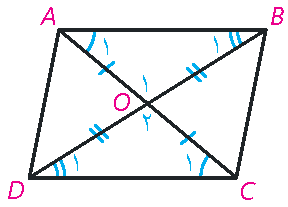
\includegraphics{"Shapes/Fasl - 3/Dars 1/qazie 4 ax.pdf"}
	\end{flushleft}
\end{minipage}
\newline

\subsection{ویژگی‌هایی از مستطیل و لوزی}
در مستطیل 
$
ABCD
$،
دو قطر را رسم می‌کنیم. از هم‌نهشتی دو مثلث 
$
ACD
$
و
$
BCD
$
می‌توان نتیجه گرفت 
$
AC = BD
$.

\begin{minipage}{.68\textwidth}
	\begin{flushleft}
		$ 
		\left. 
		\begin{array}{crr}
			\widehat{D} = \widehat{C} \\
			AD = BC \\
			CD = CD
		\end{array}
		\right\}
		\xRightarrow{\mbox{ض‌زض}} \triangle ACD \cong \triangle BCD \Rightarrow
		AC = BD
		$
		
	\end{flushleft}
\end{minipage}
\begin{minipage}{.28\textwidth}
	\begin{flushleft}
		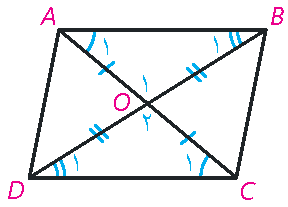
\includegraphics{"Shapes/Fasl - 3/Dars 1/qazie 4 ax.pdf"}
	\end{flushleft}
\end{minipage}
\newline

بنابراین در هر مستطیل اقطار برابرند.

اگر دو قطر یک چهار ضلعی هم‌اندازه باشند. نمی‌توان نتیجه گرفت که آن چهارضلعی مستطیل است، ولی اگر آن چهارضلعی متوازی‌الاضلاع باشد، جتما مستطیل است.

\begin{minipage}{.47\textwidth}
	\begin{flushleft}
		$ 
		\left. 
		\begin{array}{crr}
			AC = BD \\
			AD = BC \\
			CD = CD
		\end{array}
		\right\}
		\xRightarrow{\mbox{ض‌ض‌ض}} \triangle ACD \cong \triangle BCD 
		$
		\centering
		$
		\widehat{D} =\widehat{C} = 90^{\circ}
		$
		
	\end{flushleft}
\end{minipage}
\begin{minipage}{.58\textwidth}
	\begin{flushleft}
		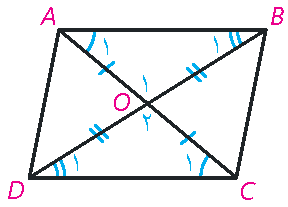
\includegraphics{"Shapes/Fasl - 3/Dars 1/qazie 4 ax.pdf"}
		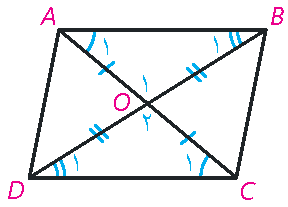
\includegraphics{"Shapes/Fasl - 3/Dars 1/qazie 4 ax.pdf"}
	\end{flushleft}
\end{minipage}

\subsection{ویژگی‌ مهمی در مثلث قائم‌الزاویه}
در هر مثلث قائم‌الزاویه ‌اندازه‌ی مینه‌ی وارد بر وتر
 \textbf{نصف}
 اندازه‌ی وتر است.
 
 \begin{minipage}{.65\textwidth}
 	\centering فرض: 
 	$
 	\widehat{A} = 90^{\circ} \; , \; BM = MC
 	$
 	\qquad حکم:
 	$ 
 	AM = \frac{BC}{2}
 	$
 	\newline
 	
 	ابتدا به اندازه‌ی 
 	$
 	AM
 	$
 	خط 
 	$
 	AM
 	$
 	را ادامه می‌دهیم و نقطه‌ی $D$ را مشخص می‌کنیم. نقطه‌ی $D$ را به موازات $AC$ به $B$ و به موازات $AB$ به $C$ متصل می‌کنیم 
 	\begin{flushleft}
 		$ 
 		\left. 
 		\begin{array}{crr}
 			BM = CM \\
 			AM = DM 
 		\end{array}
 		\right\}
 		\Rightarrow \mbox{متوازی‌الاضلاع } ABCD \xRightarrow{\widehat{A} = 90^{\circ}} \mbox{مستطیل } ABCD
 		$
 		\begin{flushright}
 			$
 			AD = BC
 			$
 			
 			$
 			BM = CM = AM = DM \Rightarrow AM = \frac{BC}{2}
 			$
 		\end{flushright}
 	
 	
 	\end{flushleft}
 \end{minipage}
 \begin{minipage}{.28\textwidth}
 	\begin{flushleft}
 		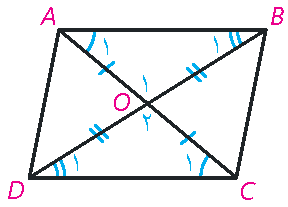
\includegraphics{"Shapes/Fasl - 3/Dars 1/qazie 4 ax.pdf"}
 	\end{flushleft}
 \end{minipage}
 
 

\subsection{ویژگی‌هایی که فقط در لوزی برقرارند}
اقطار لوزی
	$ABCD$
  را رسم می‌کنیم. چون لوزی متوازی‌الاضلاع است، اقطار منصف یکدیگرند. 
$
	\triangle ABD
$
نیز متساوی‌الساقین است.

نقطه تلاقی دو قطر را
 	$H$
  می‌نامیم، در مثلث
  	$ABD$،
   	$AH$
     عمودمنصف
	$BD$
      و روی نیمساز 
$
	\widehat{A}
$
است.

بنابراین؛
\newline \smallskip

{\large در هر لوزی اقطار \textbf{عمودمنصف} یکدیگیر و روی \textbf{نیمساز} زوایا هستند.}

\subsection{ذوزنقه}

\section{مساحت و کاربردهای آن}

\chapter{تجسم فضایی}

\section{خط، نقطه و صفحه}

\section{تفکر تجسمی}


\end{document}